\section{Events-Vis: Method}

%
The initial adaptation was to transform the heatmap used in the literature into a scatter plot,
%
so it was possible to represent events as rectangles with different widths and heights, instead of fixed grid size, and use these two properties to represent data features.
%
In the scatter plot, time will be mapped to the horizontal axis, and the width of rectangles will represent the temporal size of events; space will be mapped to the vertical axis, with the height of rectangles representing the area of the region of the event.
%

The horizontal axis can be easily created with a linear scale based on the time information of start and end of events, so the width would be representing the duration of an event. 
%
To create the vertical axis, it was necessary to transform the 2D information to 1D, and differently from the literature, a projection could not be applied directly to events because they are not single points.
%
A solution to this task was a development of a method for vertical positioning that initially uses a projection, and after that try to adjust for the intersection between events.

\begin{figure}[th]
    \centering
    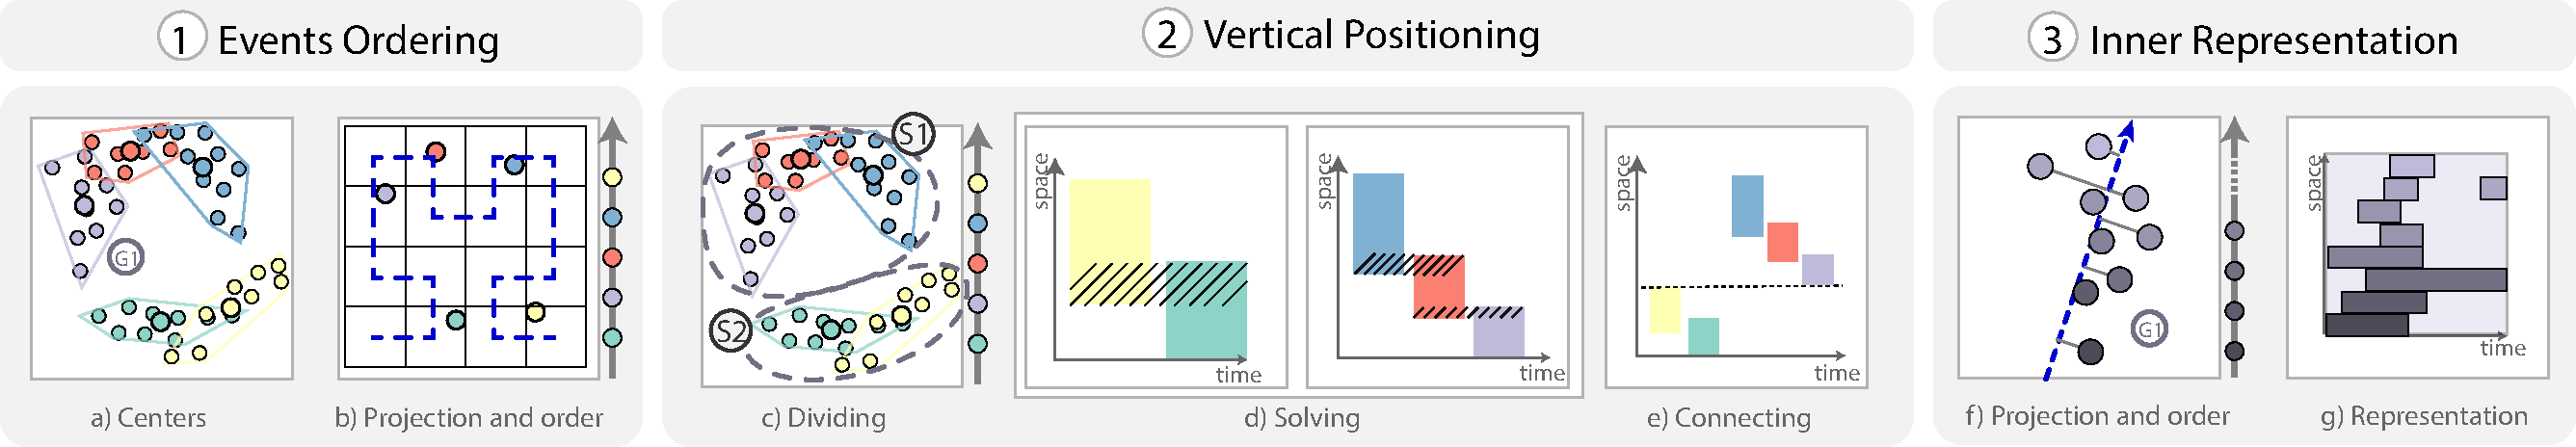
\includegraphics[width = \textwidth]{src/imgs/pipeline.pdf}
    \caption{Source: elaborated by author. Events-Vis pipeline: 1) events are initially ordered, 2) based on this ordering, on the area, and area of intersections, the rectangles are positioned vertically, 3) the inner structure of rectangles is represented inside each one.}
    \label{fig:pipeline}
\end{figure}

The pipeline of this method is exhibited in Figure~\ref{fig:pipeline}, and can be divided into three steps: 1) the center position of events is computed and events are ordered based on a projection, 2) the rectangles representing events are positioned vertically and 3) the inner points of each event are represented inside rectangles. Each step will be detailed in the following sections.

\textbf{Algorithm input} Consider that we have a set of $n$ events denoted by $(e_i)|_{i = 1}^n$, if events are composed by a set of points, it can be computed a convex hull to represent the spatial span of points, otherwise, events must also include information of a polygon in space. 
%
For each, there is a measure of area of the spatial span $a_i \in \mathbb{R}^+$, for each pair of events $(e_i, e_j)$ there is also a measure of the area of spatial intersection $w_{i, j} \in \mathbb{R}^+$.

\subsection{Events Ordering}

To project events from 2D to 1D it is possible to use a point as a representative of each event, and project this point to obtain a projection of events. 
%
The representative point can be the mean of points if there is a set of points or can be the mass center of the spatial shape of the event.
%
From this projection, it is obtained an ordering of events, if the projection of $e_i$ was smaller than the projection of $e_j$, it will denote that $e_i < e_j$.
%
On Figure~\ref{fig:pipeline} a) there are example events and the respective convex hulls, that have their center projected on b), obtaining the exhibited order.

%
The projection methods used were the methods described in section \ref{seq:space-transformation},
%
the result of the visualization is highly dependent on the choice of projection method, so it is necessary an evaluation of the considered methods.
 
\subsection{Vertical Positioning}

In the second step, the order of events will be used to position the rectangles on the vertical axis. 
%
As the horizontal direction represents time, in this step the rectangles can be simplified to segments perpendicular to the x-axis, $s_i$ being the segment of event $e_i$. Consider that the index of events is based on their order, i.e., if $i < j$  the order of events obtained in the projection step is $e_i < e_j$. 
%

%
Let $(0, y_i)$ be the mean point of segment $s_i$ in the Cartesian plane and $h_i$ be its length, i.e., the segment $s_i$ starts at the point $(0, y_i - \frac{h_i}{2})$ and ends at the point $(0, y_i + \frac{h_i}{2})$. 
%
The order of the segments $(s_i, s_j)$ is defined by the order of values $(y_i, y_j)$.
%
For a pair of segments $(s_i, s_j)$ it is also defined the value $I_{i,j}$ is the value of geometrical intersection between them. Geometrically, if there is no intersection, $I_{i, j} = 0$, if there is an intersection, it is valid the formula:
\begin{equation*}
I_{i, j} = \frac{h_i + h_j}{2} - |y_i - y_j|    
\end{equation*}

If there isn't geometric intersection, $\frac{h_i + h_j}{2} - |y_i - y_j| < 0$, so unifying both cases:

\begin{equation}
I_{i, j} = \max\left\{0, \frac{h_i + h_j}{2} - |y_i - y_j|\right\}    
\end{equation}

It is expected that the order of events obtained is able to preserve the neighborhoods, i.e., 
%
if the segments show the same order of events, for each $s_i$ the neighborhood of segments will be the same (or close) of the neighborhood of $e_i$, so this order will be preserved when placing segments vertically. 
%
As already said, $h_i$ should represent the area of events, so it is set to $h_i = a_i$ and for each pair of segments $(s_i, s_j)$ it is also desired that the intersection of segments is close to the value of $w_{i, j}$. 
%
For each pair of events, we can represent the distance between events and segments intersections with quadratic distance or absolute value.
%
Consider the loss defined by:

\begin{equation}
    \mathcal{L}(y_1, \dots, y_n) = \sum_{i = 1}^n \sum_{j = i+1}^n g(w_{i, j} - I{i,j})
    \label{loss_intersection_quadratic}
\end{equation}
%

With $g: \mathbb{R} \to \mathbb{R}^+$ being a norm,  i.e., $g(x) > 0 \quad \forall x \neq 0$, $g(0) = 0$ and $g(x) < g(y)$ if $x < y$, such as $g(x) = x^2$ or $g(x) = |x|$.

For the solution of this problem, it was used different methods of optimization, it was proposed a greedy heuristic and convex optimization programs.

\subsubsection{Greedy heuristic}

The greedy heuristic is an intuitive and fast solution for the problem of vertical positioning, this method consists of iterating over the ordered events and placing one at a time with greedy decisions.
%

To compute values $y_1, \dots, y_n$ such that the loss is close to an optimal solution, the greedy steps minimize individual terms of the sum. 
%
Iterating over events $e_1, \dots, e_n$, at a iteration with $e_{i}$ and the previous solution for $e_{i-1}$,  a greedy decision is used to try to minimize the loss considering only this step, and the segment $s_i$ is positioned in a manner that the $I_{i-1,i} = w_{i-1, i}$, i.e., the loss is $0$ for this particular pair of consecutive events.

%
In more detail, the greedy method computes:

\begin{equation}
    \begin{split}
        y_1 &= \dfrac{h_1}{2} \\
        y_i &= y_{i -1} + \frac{h_i + h_{i-1}}{2} - w_{i-1, i} \quad i = 2, \dots, n   
    \end{split}
\end{equation}

From the second line we can obtain:

\begin{equation}
\begin{split}
     y_i &= y_{i -1} + \frac{h_i + h_{i-1}}{2} - w_{i-1, i} \implies \\
     I_{i-1,i} &= \frac{h_i + h_{i-1}}{2} - (y_i - y_{i -1})  = w_{i-1, i}  \implies \\
     I_{i-1,i} - w_{i-1, i}  &= 0
\end{split}
\end{equation}

Focusing on minimizing the loss between consecutive events, there is no guarantee for the intersections of events that are not consecutive are well represented.
%
The results depend on how well the ordering of events keeps events that intersect in consecutive positions.
%
A visual interpretation of the greedy method is available on Fig.~\ref{fig:pipeline} d), the events are placed starting on the x-axis, and following the obtained order, they are positioned according to the intersection values. 

\subsubsection{Convex optimization}

The loss present in ~\ref{loss_intersection_quadratic} is convex and most of the desired restrictions to the vertical positioning problem can be also represented  as convex functions, so convex optimization methods can be used.
%

The convex formulation contains many variations, the first is on the set of decision variables.
%
The values $y_{i} \in \mathbb{R}$ that are the position of segments is the decision variable common to all variations, 
%
but the height of segments $h_i$ can be also a decision variable if the users consider that to get a better representation of the intersections, the optimization can change the heights of rectangles.
%

%
The constraints on variables $y_i \in \{1, \dots, n \}$ are to guarantee the order obtained in the projection step, there is a total of $n-1$ constraints with the form:

\begin{equation}
    y_{i - 1} \leq y_i \quad \quad \forall i \in \{2, \dots, n\}
\end{equation}
\label{eq:order-constraint}

%
When optimizing the heights, it is interesting to define thresholds on how distant from the original area of the events it can be, the parameters are constant that are multiplied to the area to obtain the thresholds, let call it as $\tau_1$ and $\tau_2$, the $n$ restrictions are:

\begin{equation}
    \tau_1 a_i \leq h_i \leq \tau_2 a_i \quad \quad \forall i \in \{2, \dots, n\}
\end{equation}
\label{eq:height-constraint}

Generally, good options are the pair $(1 - c,  1 + c)$ with $0 < c < 1$ so the height cannot have a difference from the area bigger than $(c*100)\%$ of the area value.
%

Now it is necessary to define the objective function, 
%
it will be the error that needs to be minimized and can be separated into two sums, the first is only is used when the height is optimized and is the difference between $h_i$ and $a_i$. It is defined as the sum of the quadratic differences
%

\begin{equation}
    \mathcal{L}_h = \sum_{i = 1}^n (h_i - a_i)^2
\end{equation}

Now we need to consider the sums of differences between $w_{i, j}$ and $I_{i, j}$.
%
One method that is able to represent the $\max$ function present in the definition of the value $I$ is to use binary decision variables together with the real variables. Consider it is desired to minimize $f(c)$ with $c = \max \{x, y\}$, $x, y$ decision variables. Using a binary variable $b \in \{0, 1\}$ and an value $M$ that is bigger than the $\max \{ | x -y |\}$ in the feasible set, it is defined the restrictions:

\begin{equation}
    \begin{split}
        &c \geq x \\
        &c \geq y \\
        &c \leq x + bM \\
        &c \leq y + (1- b)M 
    \end{split}
    \label{binary_max_trick}
\end{equation}

When $x < y$, the only value of $b$ that satisfies the restrictions is $1$:

\begin{equation*}
    \begin{split}
        &c \geq x \\
        &c \geq y \\
        &c \leq x + M \\
        &c \leq y  
    \end{split}
\end{equation*}

Because $x + M > y$ and the result is $c \leq y, c \geq y \implies c = y$. When $x > y$, the only value of $b$ that satisfies is $0$:

\begin{equation*}
    \begin{split}
        &c \geq x \\
        &c \geq y \\
        &c \leq x  \\
        &c \leq y + M 
    \end{split}
\end{equation*}

In a similar manner, it is valid that $c = x$. When $x = y$, $b$ can be $0$ or $1$, which implies that $c = x$ and $c = y $ are both valid solution to the system. So:

\begin{equation*}
    c = 
    \begin{cases}
      x, \text{ if } x \geq y  \\ 
      y, \text{ if } y > x
    \end{cases}
     = \max \{x, y \}
\end{equation*}

Using this same idea of \ref{binary_max_trick}, a decision variable $\tilde I_{i, j}$ can be defined to represent the value of $I_{i,j}$, for each $i < j$ it is add the following constraints:

\begin{equation}
    \begin{split}
        &\tilde I_{i,j} \geq 0 \\
        &\tilde I_{i,j} \geq \left (
        \dfrac{h_i + h_j}{2} - (y_j - y_i) \right)\\
        &\tilde I_{i,j} \leq b_{i, j}M \\
        &\tilde I_{i,j} \leq \left( \dfrac{h_i + h_j}{2} - (y_j - y_i) \right) + (1- b_{i, j})M \\
        &b_{i, j} \in \{0, 1 \}
    \end{split}
    \label{eq:intersection_trick_constraints}
\end{equation}

This set of constraints is the same when $h_i$ is a decision variable or a fixed constant.

For each pair of events $(i, j)$, we sum the quadratic difference between intersections. 
%
To obtain better results, each term is multiplied by the biggest area between $(a_i, a_j)$ so that events with bigger areas will not have more importance when minimizing the errors.

\begin{equation}
    \mathcal{L}_I = \sum_{i = 1}^n \sum_{j = i + 1}^n (\tilde I_{i, j} - w_{i, j}) \dfrac{1}{\max \{ a_i, a_j\} }
\end{equation}

Another option for this loss is to ignore the error when $w_{i, j} = 0$, the interpretation of this modeling is that we desire to represent an intersection between segments when there is in the original space $(w_{i, j} > 0)$, 
%
but if events do not intersect each other, it is not important if the segments will intersect themselves or not.
%
This new loss functions uses an indicator variable that is $0$ when $w_{i, j} = 0$.
We will refer to it as \textit{"ignore-zeros"} and the previous version as \textit{"optim-zeros"}.

\begin{equation}
    \mathcal{L}_I' = \sum_{i = 1}^n \sum_{j = i + 1}^n (\tilde I_{i, j} - w_{i, j}) \dfrac{ \mathbb{I}[w_{i, j} = 0 ]}{\max \{ a_i, a_j\}}
\end{equation}

The final loss will depend on the variation of the method. If the height is optimized, it is the sum of $\mathcal{L}_I$ or $\mathcal{L}_I'$ with $\mathcal{L}_h$, 
%
and in that case, it is used a parameter $\lambda \in \mathbb{R}^+$ to set importance for the different terms:

\begin{equation}
    \mathcal{L} = \mathcal{L}_I + \lambda \mathcal{L}_h
\end{equation}

To recall, the different variations for the optimization method is if the heights will be optimized or not, the parameters $(\tau_1, \tau_2)$, the choice between losses $L_I$ or $L_I'$ and the parameter $\lambda$.

As there is a quadratic function on the objective, and we made use of binary variables, to solve this problem it was used methods of Mixed Integer Quadratic Programming.

\subsubsection{Problem decomposition}

To decrease the processing time for the solution, it was considered that one way was dividing the problem of vertical positioning into subproblems.
%
Considering that are two subsets of events $S_1$ and $S_2$, and no event from one subset had an intersection with events of the other. Ignoring the restrictions to preserve the order, the optimal solution for the problem would be to solve the vertical positioning in each subset and concatenate the solutions of the subsets of segments, placing them one after the other.
%

%
Based on this idea, before applying our algorithms, events were grouped into subsets ($S_1, S_2, \dots, S_m$).
%
Each subset only contains events that intersect themselves; more formally, $e_i$ and $e_j$ are on the same subset if there is a sequence of events ($e_i, e_{i_1}, e_{i_2}, \dots, e_{i_k}, e_j $) where each consecutive pair has a non-empty spatial intersection, $w_{i,i_1} > 0, \dots, w_{i_k,j} > 0$. 
%
As shown in Figure~\ref{fig:subset-events}, the subsets can be interpreted visually, they are chains of events that intersect at least one of the other events in the group.

\begin{figure}
    \centering
    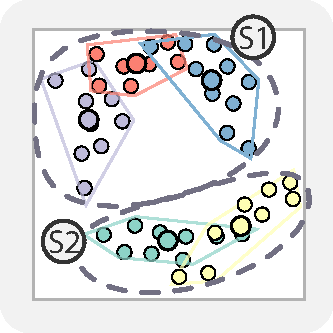
\includegraphics[width = 0.3\textwidth]{src/imgs/subset-events.pdf}
    \caption{Source: elaborated by author. Example of separating events in two subsets that intersect themselves.}
    \label{fig:subset-events}
\end{figure}

Then, for each subset separately the vertical positioning problem is solved, and the result is obtained by vertically concatenating the results of each subset. To realize this concatenation, it is first identified an order of subsets.
%
It is defined that $S_j < S_k$ if $\min \{e_i | e_i \in S_j \} < \min \{ e_i | e_i \in S_k \}$, i.e., the order of subsets is defined by their event with smaller projection.
%
On the example, the order of the green event is the minimum for $S_1$ and the purple event is the minimum for subset $S_2$, so the order of this pair of subsets is based on the order between events green and purple.

%
With this order,
%
the next step is to iterate over subsets $S_1, \dots, S_m$. The first subset is placed on the Cartesian plane such that the segment with lowest start point, $p_{start} = \min \{ y_i - \frac{h_1}{2} | e_i \in S_1 \}$, is on the line $y = 0$, it is done by subtracting $p_{start}$ for each $y_i$ that $e_i \in S_1$.
%
For each of the following iterations with $S_{i - 1}$ and $S_i$, it is calculated the highest end point of segments from $S_{i - 1}$, $p_{end} = \max \{ y_j + \frac{h_j}{2}| e_j \in S_{i - 1}\}$ and the lowest start point of segments from $S_i$, $p_{start} = \max \{ y_j - \frac{h_j}{2}| e_j \in S_{i}\}$, then let $d = p_{start} - p_{end}$ and subtract $d$ from each $y_j$ that $e_j \in S_i$, the obtained result is that segments from $S_i$ is just after segments from $S_{i-1}$.
%
In Fig.~\ref{fig:pipeline} e), the two subsets are concatenated and a dashed line marks their connection. 

\subsection{Inner Representation}

Finally, if there is an inner structure for each event, in our specific case where events are groups of points,
%
this structure contains important information and will also be displayed in the final plot.
%
Inside each rectangle, the method represents the inner points trying to reproduce an "event space".
%
To obtain that result, a similar process of positioning events is applied, but now these points will not have area.
%
For each event, we project the points using one of the previously mentioned methods, the transformation is fitted for each of the events, and not for all points of all events. 
%
The vertical order of the inner points inside the rectangle is based on this projection. 

%
We represent each point as a rectangle, if it has a time duration, we compute the width of this rectangle proportional to this value; otherwise (i.e., it is an instant), it will have a fixed size. 
%
The height of these inner rectangles is equal to the height of the event rectangle divided by the number of points, so events with more points will have inner rectangles with smaller heights.

%
In our example, the event \textit{G1} from Fig.~\ref{fig:pipeline} a), has its inner representation better detailed in Figure~\ref{fig:inner-representation}.

\begin{figure}[h]
    \centering
    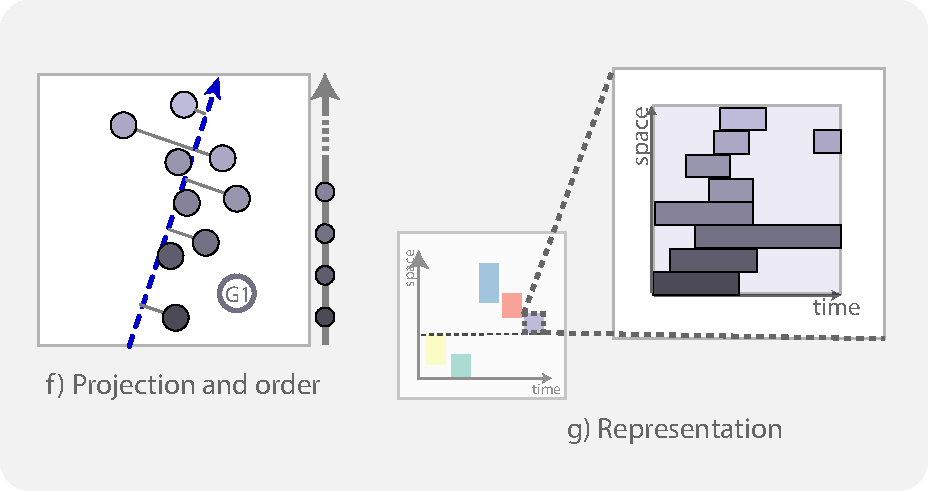
\includegraphics[width = 0.7\textwidth]{src/imgs/inner-representation.pdf}
    \caption{Source: elaborated by author. Example of inner representation of an event.}
    \label{fig:inner-representation}
\end{figure}


